Neste capítulo são apresentados os resultados
da simulações numéricas para o escoamento sanguíneo
em uma artéria coronária.
O raio do lúmen da artéria coronariana é $R=0.0015m$,
a viscosidade é $\mu=0.0035Pa.s$ e
a massa específica é $\rho=1060kg/m^3$ como sugerido
por Bozsak, Chomaz e Barakat (2014) \cite{bozsak2014}. De acordo com Kessler et al. (1998) \cite{kessler1998},
a velocidade do sangue na artéria coronária é $u=12cm/s$.
Dessa forma, o número de Reynolds utilizado será $Re=54.5$.\par
A equação de Navier-Stokes
é utilizada segundo a formulação corrente-vorticidade
com o acoplamento da equação de transporte de espécie
química para quatro geometrias propostas por Wang et al. (2017) \cite{wang2017},
porém modificadas para coordenadas cartesianas como apresentado
na \ref{coronary artery geo}.
Na seção \ref{canal curvado}, a artéria coronária com aterosclerose é modelada
como um escoamento em um canal curvado. Na seção \ref{canal curvado com stent},
é apresentado a simulação para a artéria coronária com aterosclerose
e com stent farmacológico colocado para diversos \textit{Schmidt},
tais como $Sc=1$ e $10$. Na seção \ref{canal real}, é apresentado
a simulação de uma artéria coronária real com aterosclerose e na
seção \ref{canal real com stent}, a artéria coronária real com aterosclerose e com stent
farmacológico é simulado com diversos números de \textit{Schmidt}
como no caso da seção \ref{canal curvado com stent}. 
Devido a simetria, apenas a metade do domínio foi
simulado. A visualização da simulação foi feita pelo software livre \textit{Paraview}
proposto por Henderson (2007) \cite{paraview}.


\begin{figure}[H]
     \centering
     \begin{minipage}{.45\linewidth}
      \centering
      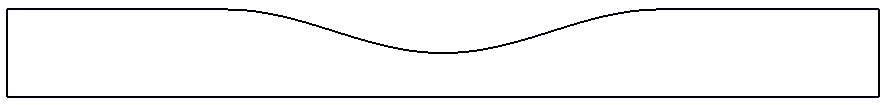
\includegraphics[scale=0.22]{./02_chaps/cap_solution/figure/Curved.png}\\
      (a)
     \end{minipage}%
     \begin{minipage}{.45\linewidth}
      \centering
      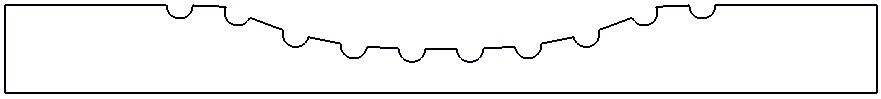
\includegraphics[scale=0.22]{./02_chaps/cap_solution/figure/CurvedStrut.png}\\
      (b)
     \end{minipage}
     \begin{minipage}{.45\linewidth}
      \centering
      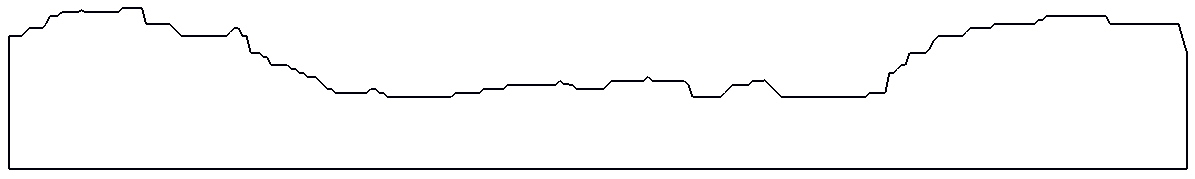
\includegraphics[scale=0.16]{./02_chaps/cap_solution/figure/Real.png}\\
      (c)
     \end{minipage}%
     \begin{minipage}{.45\linewidth}
      \centering
      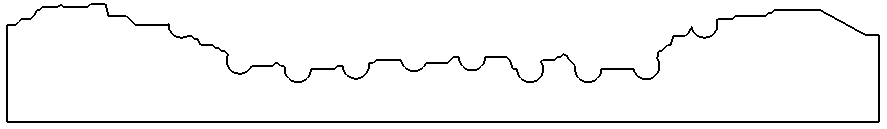
\includegraphics[scale=0.22]{./02_chaps/cap_solution/figure/RealStrut.png}\\
      (d)
     \end{minipage}
     \medskip
     \caption{Geometria não dimensional para escoamento sanguíneao em artéria coronária.
     O raio é $R=1$ e o comprimento do canal é $L=10R$.
     (a) Canal Curvado
     (b) Canal Curvado com Stent
     (c) Canal Real e
     (d) Canal Real com Stent.}
     \label{coronary artery geo}
\end{figure}

\newpage
\medskip
\noindent
As condições de contorno utilizadas nessas simulações foram:

\begin{itemize}
     \item \textit{condição de entrada}:
      a componente normal da velocidade é $v=0$ enquanto a componente tangencial da velocidade é $u = 1$. 
      A função de corrente também é especificada e seu valor é definido segundo a equação da continuidade 
      para um fluido incompressível. Dessa forma, seu valor será $\psi = y$.
      A derivada da concentração possui o valor nulo $\partial c / \partial n = 0$.


     \item \textit{condição de não escorregamento}: esta condição é utilizada na parede superior, 
      onde todas as componentes da velocidade são especificadas
      com os valores $u=0$ e $v=0$.
      A função de corrente também é especificado com o valor de $\psi=1$. A derivada da concentração
      possui o valor nulo $\partial c / \partial n =0$.

     \item \textit{condição de saída}: O valor da função de corrente é especificado $\psi=y$. As derivadas das
     componentes tangencial e normal da velocidade e da concentração possuem o 
     valor nulo, isto é,
      $\partial u/\partial n = 0$,
      $\partial v/\partial n = 0$ e
      $\partial c / \partial n =0$ respectivamente.

     \item \textit{condição de livre escorregamento}: esta condição é utilizada no eixo de simetria.
      A componente normal da velocidade e a função de corrente possuem seus valores especificados,
      tais como $v=0$ e $\psi=0$ respectivamente. A derivada da componente tangencial da velocidade
      e a derivada da concentração possuem também o valor nulo $\partial u/\partial n = 0$ e 
      $\partial c/\partial n = 0$ respectivamente.

     \item \textit{condição de espécie química}: esta condição é utilizada no stent farmacológico, 
      onde todas as componentes da velocidade são especificadas
      com os valores $u=0$ e $v=0$.
      A função de corrente e a concentração também são espeficados com os valores de $\psi=1$
      e $c=1$ respectivamente.
\end{itemize}

\medskip
\noindent
Conforme foi informado nas seções anteriores, a condição de contono do campo de vorticidade
é calculado através do algoritmo de solução como apresentado na \ref{solution algorithm}.

\newpage
